\subsection{Mathias}
\begin{figure}[hbtp]
  \centering
  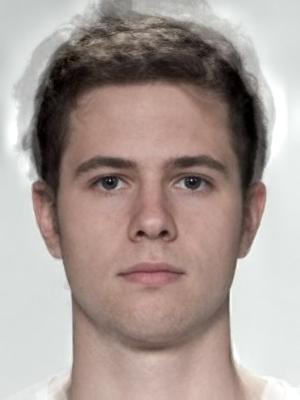
\includegraphics[]{mathias.jpg}
  \caption{Picture associated with the persona \enquote{Mathias}. Copyright the Face Research Lab. Used with permission.}\label{fig:mathias}
\end{figure}
\noindent\textbf{Basic information}

\begin{itemize}
\item 21 years old
\item Mechanical engineering student
\item Introvert
\item Thoughtful person that can be shy at times
\end{itemize}

Mathias is intelligent, logical and not very good with social interaction. Mathias, like most of his peers, likes going to a bar and having a beer or two after a productive week and this week was going to be no different. Mathias goes to his favourite bar, but soon finds that the music is not fitting to his mood. Normally, this would be a deal breaker for Mathias, and he would find another bar for the night, as he was not really comfortable going to the bartender and requesting music he likes. Fortunately Mathias had just learned about openPlaylist. Mathias opens the app and finds that it is only the next couple of tracks that he dislikes, so he decides to vote for tracks which he does like and stays at the bar after all.
